\subsection{Konsep dan Struktur Blockchain}
\label{subsec:konsep-struktur-blockchain}

Blockchain adalah sebuah sistem pencatatan data terdistribusi yang tersusun atas serangkaian blok, di mana setiap blok menyimpan daftar transaksi secara lengkap seperti \textit{public ledger} konvensional. Data disimpan secara terdistribusi pada banyak \textit{node} dalam jaringan, sehingga tidak ada entitas terpusat yang mengontrol keseluruhan sistem. Setiap blok yang memuat transaksi harus divalidasi menggunakan mekanisme konsesus tertentu sebelum ditambahkan ke dalam rantai blok. Proses konsensus melibatkan mayoritas dari \textit{node} untuk menyetujui atau menolak \textit{state} baru dari \textit{ledger}, sehingga menjamin integritas dan keaslian dari data \parencite{zheng2018blockchain,nofer2017blockchain}.

Pada sistem Blockchain klasik, seperti pada gambar \ref{image:struktur-blockchain}, setiap blok umumnya memiliki daftar transaksi yang lengkap, ditambah dengan \textit{timestamp} pembuatan blok, nilai \textit{hash} dari blok sebelumnya ("\textit{parent}"), dan sebuah \textit{nonce}, yang adalah sebuah angka acak yang digunakan untuk mekanisme verifikasi \textit{hash}.
Konsep ini memastikan integritas dari Blockchain dimulai dari blok pertama ("\textit{genesis block}") sampai ke blok terakhir yang akan terus bertambah, karena setiap perubahan data akan membuat nilai \textit{hash} dari sebuah blok berubah, yang harus dipropagasikan ke setiap blok setelahnya.

Aspek penting dari sebuah Blockchain adalah proses konsensus yang dimilikinya, yang dilakukan dengan mengikuti sebuah kumpulan aturan dan prosedur untuk mempertahankan himpunan fakta yang koheren diantara beberapa \textit{participating nodes}. Terdapat banyak mekanisme konsensus yang berbeda yang digunakan dalam \textit{Blockchain network} yang berbeda. Dalam kasus \textit{Bitcoin}, \textit{ledger} yang dianggap \textit{ledger} yang \textit{valid} adalah \textit{ledger} dengan \textit{chain} terpanjang (\textit{longest chain}) \parencite{swanson2015consensus}.

\begin{figure}[ht]
	\centering
	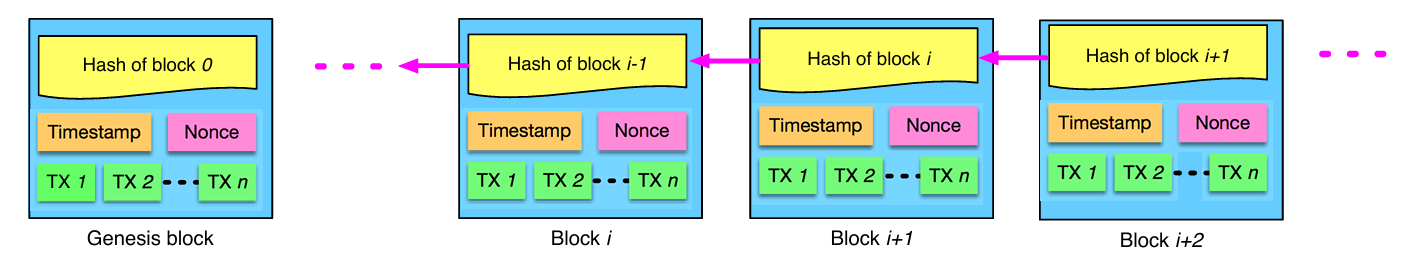
\includegraphics[width=1\textwidth]{resources/chapter-2/struktur-blockchain.png}
	\caption{Struktur blok di dalam Blockchain \parencite{zheng2018blockchain}}
	\label{image:struktur-blockchain}
\end{figure}

Struktur klasik dari sebuah blok pada Blockchain terdiri dari \textit{block header} dan \textit{block body} seperti pada Gambar \ref{image:struktur-blok}. Secara spesifik, \textit{block header} terdiri dari:

\begin{enumerate}
	\item \textit{Block Version}: mengindikasikan set dari aturan validasi yang diikuti.
	\item \textit{Parent Block Hash}: 256-bit \textit{hash} dari blok sebelumnya.
	\item \textit{Merkle Tree Root}: hasil \textit{hash} dari seluruh transaksi pada blok menggunakan mekanisme \textit{Merkle Tree}.
	\item \textit{Timestamp}: \textit{timestamp} saat ini dalam detik sejak 1970-01-01T00:00 UTC.
	\item \textit{nBits}: target \textit{hash} saat ini dalam format \textit{compact}.
	\item \textit{nonce}: \textit{number used only once}, sebuah angka yang digunakan untuk menambahkan tingkat keacakan dari nilai \textit{hash}.
\end{enumerate}

\begin{figure}[ht]
	\centering
	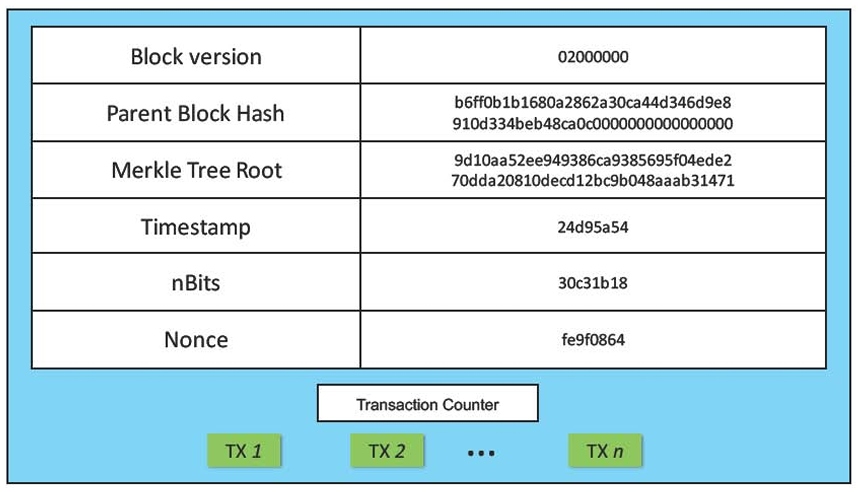
\includegraphics[width=0.7\textwidth]{resources/chapter-2/struktur-block.png}
	\caption{Struktur blok \parencite{zheng2018blockchain}}
	\label{image:struktur-blok}
\end{figure}